\documentclass[10pt]{beamer}
\usepackage[english]{babel}
\usepackage[utf8]{inputenc}
\usepackage[T1]{fontenc}
\usepackage{helvet}
\usepackage{lipsum}  
\usepackage{graphicx}
\usepackage{subcaption}

%-------------------------------------------------------
% INFORMATION IN THE TITLE PAGE
%-------------------------------------------------------

\newcommand{\cstitle}{\textbf{Neoantigen Detection Using Transformers and Transfer Learning}
	\subtitle[]{Tésis de doctorado}}
\newcommand{\cscourseCode}{PACBB Doctoral Consortium}
\newcommand{\csauthor}{Ph.D.(c) Vicente Machaca Arceda}
\institute[UNSA]{Congreso Internacional de Informática y Sistemas}
\newcommand{\csemail}{vmachaca@utec.edu.pe}
\newcommand{\instituteabr}{UTEC}
\newcommand{\nameUp}{}
\date{2023}
\title[\cscourseCode]{\cstitle}
\author{\csauthor}
%%%%%%%%%%%%%%%%%

%-------------------------------------------------------
% CHOOSE THE THEME
%-------------------------------------------------------
\def\mycmd{0} % UNSA
\def\mycmd{1} % SALLE
%\def\mycmd{2} % UTEC
%-------------------------------------------------------

\if\mycmd0
\usepackage{csformat}
\newcommand{\chref}[3][blue]{\href{#2}{\color{#1}{#3}}}%

\fi

\if\mycmd1
\usetheme[]{Feather}
\newcommand{\chref}[2]{	\href{#1}{{\usebeamercolor[bg]{Feather}#2}} }
\fi

\if\mycmd2
\usetheme{UTEC2020}	
\newcommand{\chref}[3][blue]{\href{#2}{\color{#1}{#3}}}%
\fi

\newcommand{\1}{
	\setbeamertemplate{background}{
		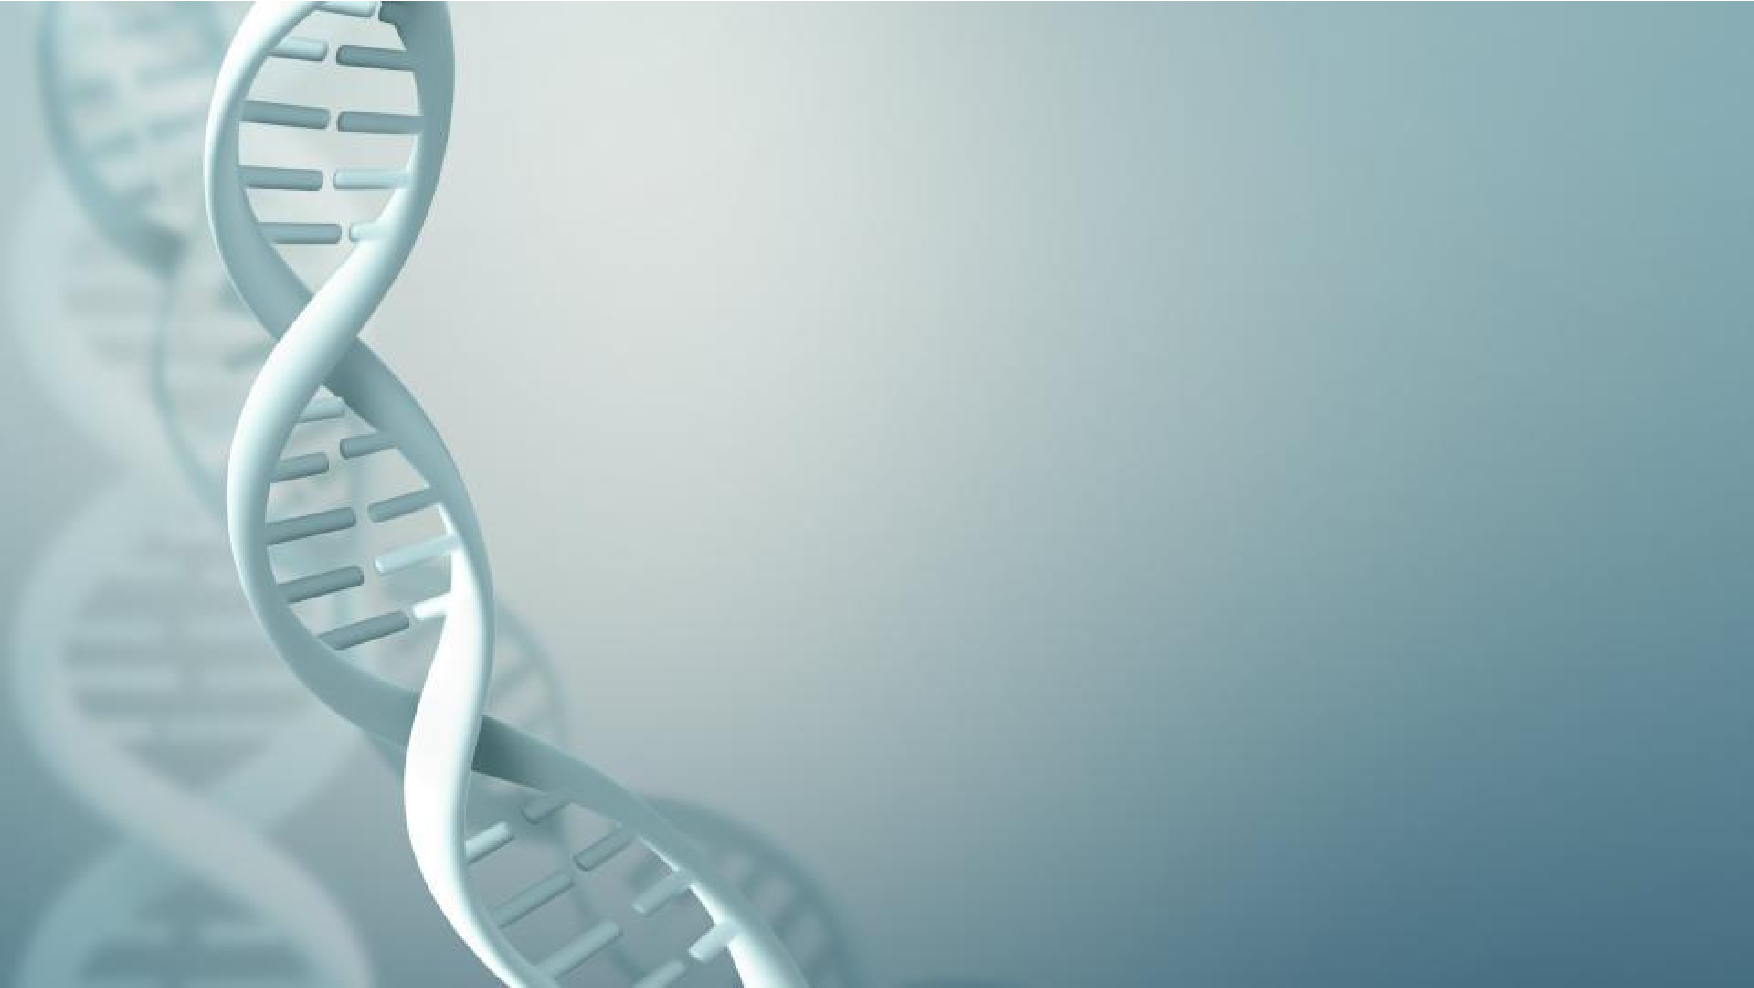
\includegraphics[width=\paperwidth,height=\paperheight]{img/1}
		\tikz[overlay] \fill[fill opacity=0.75,fill=white] (0,0) rectangle (-\paperwidth,\paperheight);
	}
}



%-------------------------------------------------------
% THE BODY OF THE PRESENTATION
%-------------------------------------------------------

\begin{document}
	
	
	\AtBeginSubsection[]
	{
		\begin{frame}
			\frametitle{Content}
			\tableofcontents[currentsubsection]
		\end{frame}
	}
	
	
	%-------------------------------------------------------
	% THE TITLEPAGE
	%-------------------------------------------------------
	
	\if\mycmd0
	\maketitle
	\fi
	
	\if\mycmd1 % MY THEME
	\1{
		\begin{frame}[plain,noframenumbering] 
			\titlepage 
	\end{frame}}
	\fi
	
	\if\mycmd2
	\begin{frame}
		\titlepage
	\end{frame}
	\fi
	%-------------------------------------------------------
	%-------------------------------------------------------
	
	
	%-------------------------------------------------------
	%-------------------------------------------------------
	\begin{frame}{Content}
		\tableofcontents
	\end{frame}
	%-------------------------------------------------------
	%-------------------------------------------------------
	
	
	%%%%%%%%%%%%%%%%%%%%%%%%%%%%%%%%%%%%%%%%%%%%%%%%%%%%%%%%%%%%%%%%%%%%%%%%%%%%%%%%%%%%%%%%%%%%%%%%%%%%%%%%%%%%%%%%
	%%%%%%%%%%%%%%%%%%%%%%%%%%%%%%%%%%%%%%%%%%%%%%%%%%%%%%%%%%%%%%%%%%%%%%%%%%%%%%%%%%%%%%%%%%%%%%%%%%%%%%%%%%%%%%%%
	%%%%%%%%%%%%%%%%%%%%%%%%%%%%%%%%%%%%%%%%%%%%%%%%%%%%%%%%%%%%%%%%%%%%%%%%%%%%%%%%%%%%%%%%%%%%%%%%%%%%%%%%%%%%%%%%
	\section{Introduction}
	%%%%%%%%%%%%%%%%%%%%%%%%%%%%%%%%%%%%%%%%%%%%%%%%%%%%%%%%%%%%%%%%%%%%%%%%%%%%%%%%%%%%%%%%%%%%%%%%%%%%%%%%%%%%%%%%
	%%%%%%%%%%%%%%%%%%%%%%%%%%%%%%%%%%%%%%%%%%%%%%%%%%%%%%%%%%%%%%%%%%%%%%%%%%%%%%%%%%%%%%%%%%%%%%%%%%%%%%%%%%%%%%%%
	%%%%%%%%%%%%%%%%%%%%%%%%%%%%%%%%%%%%%%%%%%%%%%%%%%%%%%%%%%%%%%%%%%%%%%%%%%%%%%%%%%%%%%%%%%%%%%%%%%%%%%%%%%%%%%%%
	
	
	%%%%%%%%%%%%%%%%%%%%%%%%%%%%%%%%%%%%%%%%%%%%%%%%%%%%%%%%%%%%%%%%%%%%%%%%%%%%%%%%%%%%%%%%%%%%%%%%%%%%%%%%%%%%%%%%
	%%%%%%%%%%%%%%%%%%%%%%%%%%%%%%%%%%%%%%%%%%%%%%%%%%%%%%%%%%%%%%%%%%%%%%%%%%%%%%%%%%%%%%%%%%%%%%%%%%%%%%%%%%%%%%%%
	%%%%%%%%%%%%%%%%%%%%%%%%%%%%%%%%%%%%%%%%%%%%%%%%%%%%%%%%%%%%%%%%%%%%%%%%%%%%%%%%%%%%%%%%%%%%%%%%%%%%%%%%%%%%%%%%
	\subsection{Immunotherapy to Treat Cancer}
	%%%%%%%%%%%%%%%%%%%%%%%%%%%%%%%%%%%%%%%%%%%%%%%%%%%%%%%%%%%%%%%%%%%%%%%%%%%%%%%%%%%%%%%%%%%%%%%%%%%%%%%%%%%%%%%%
	%%%%%%%%%%%%%%%%%%%%%%%%%%%%%%%%%%%%%%%%%%%%%%%%%%%%%%%%%%%%%%%%%%%%%%%%%%%%%%%%%%%%%%%%%%%%%%%%%%%%%%%%%%%%%%%%
	%%%%%%%%%%%%%%%%%%%%%%%%%%%%%%%%%%%%%%%%%%%%%%%%%%%%%%%%%%%%%%%%%%%%%%%%%%%%%%%%%%%%%%%%%%%%%%%%%%%%%%%%%%%%%%%%
	
	%-------------------------------------------------------
	%-------------------------------------------------------
	\begin{frame}{Immunotherapy to Treat Cancer}{}		
		Immunotherapy is a type of cancer treatment that helps your immune system fight cancer \cite{inmunoterapy2022}.
		
		\begin{figure}
			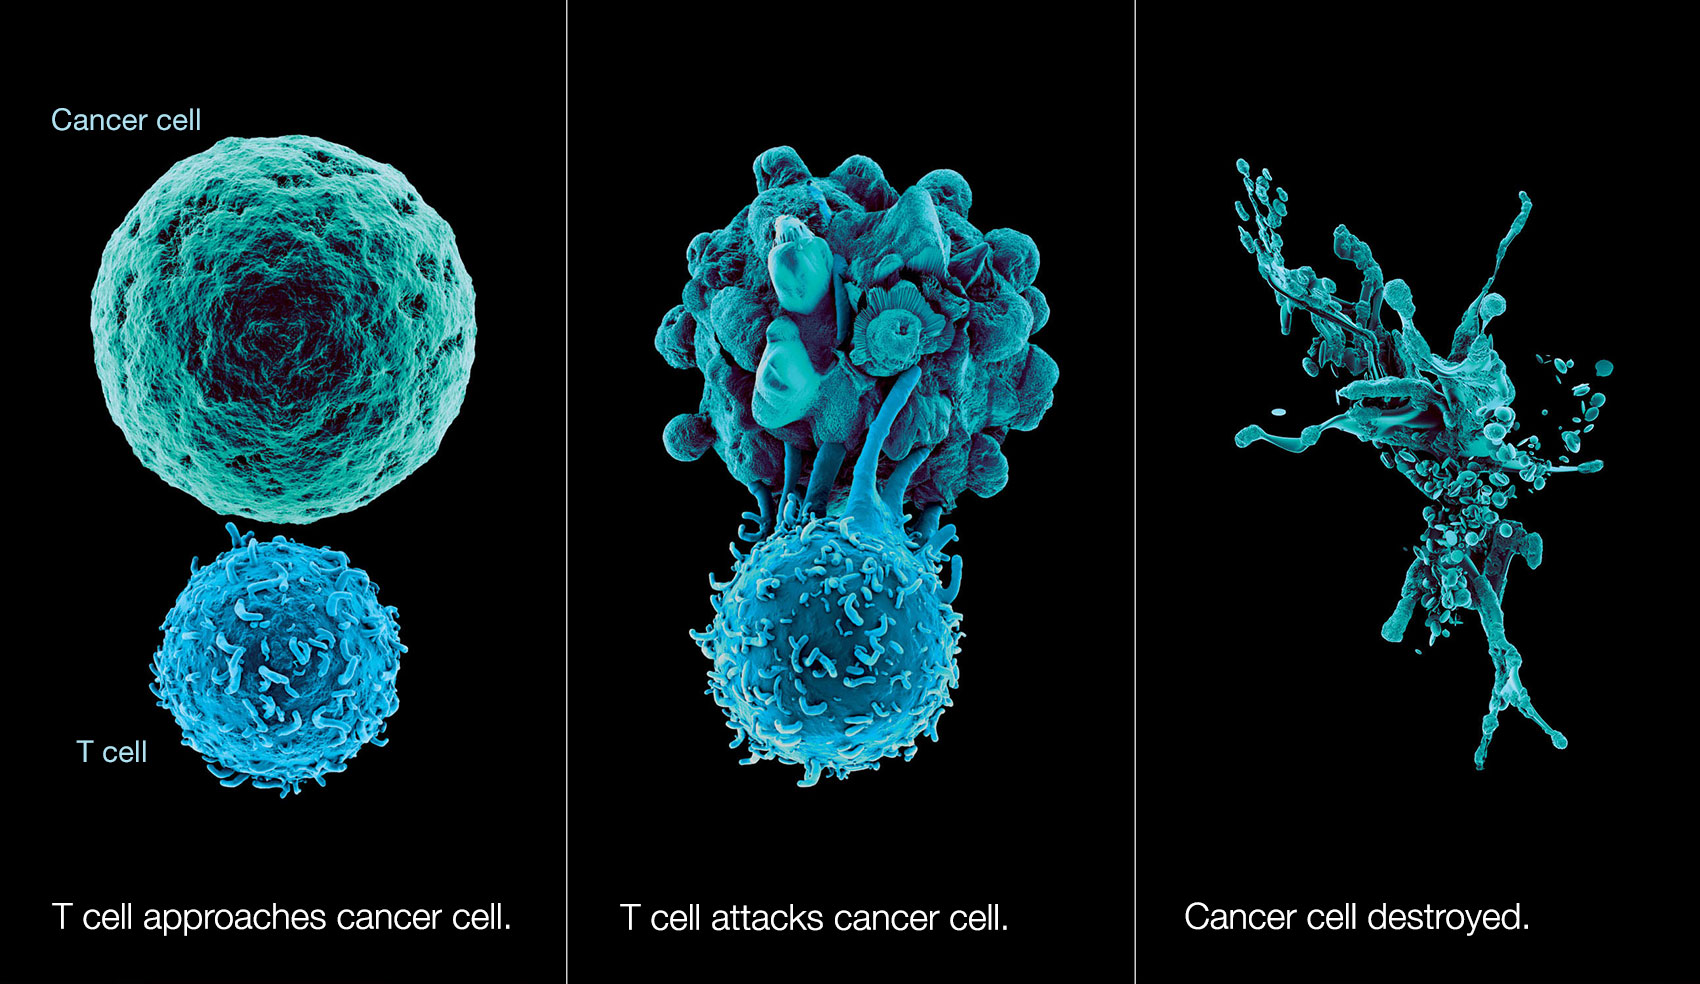
\includegraphics[width=0.85\textwidth]{../img/neoantigen/tcell}
			\caption{Example of how a T cell attack a cancer cell \cite{nortshore2022}.}
		\end{figure}		
	\end{frame}
	%-------------------------------------------------------
	%-------------------------------------------------------
	
	%-------------------------------------------------------
	%-------------------------------------------------------
	\begin{frame}{Immunotherapy to Treat Cancer}{Neoantigen}		
		\begin{block}{Neoantigen}
			A new protein that forms on cancer cells when certain mutations occur in tumor DNA. Neoantigens used in vaccines and other types of immunotherapy are being studied in the treatment of many types of cancer \cite{NCIdictionary2022, borden2022cancer}.
		\end{block} 
		\begin{block}{}
			Currently, there is a lot of methods to detect neoantigens; however, only a small number of them manage to stimulate the immune system \cite{chen2021challenges, hao2021improvement}.
		\end{block}
	\end{frame}
	%-------------------------------------------------------
	%-------------------------------------------------------
	
	
	%-------------------------------------------------------
	%-------------------------------------------------------
	\begin{frame}{Immunotherapy for Cancer}{Personalized Vaccines}	
		\begin{figure}
			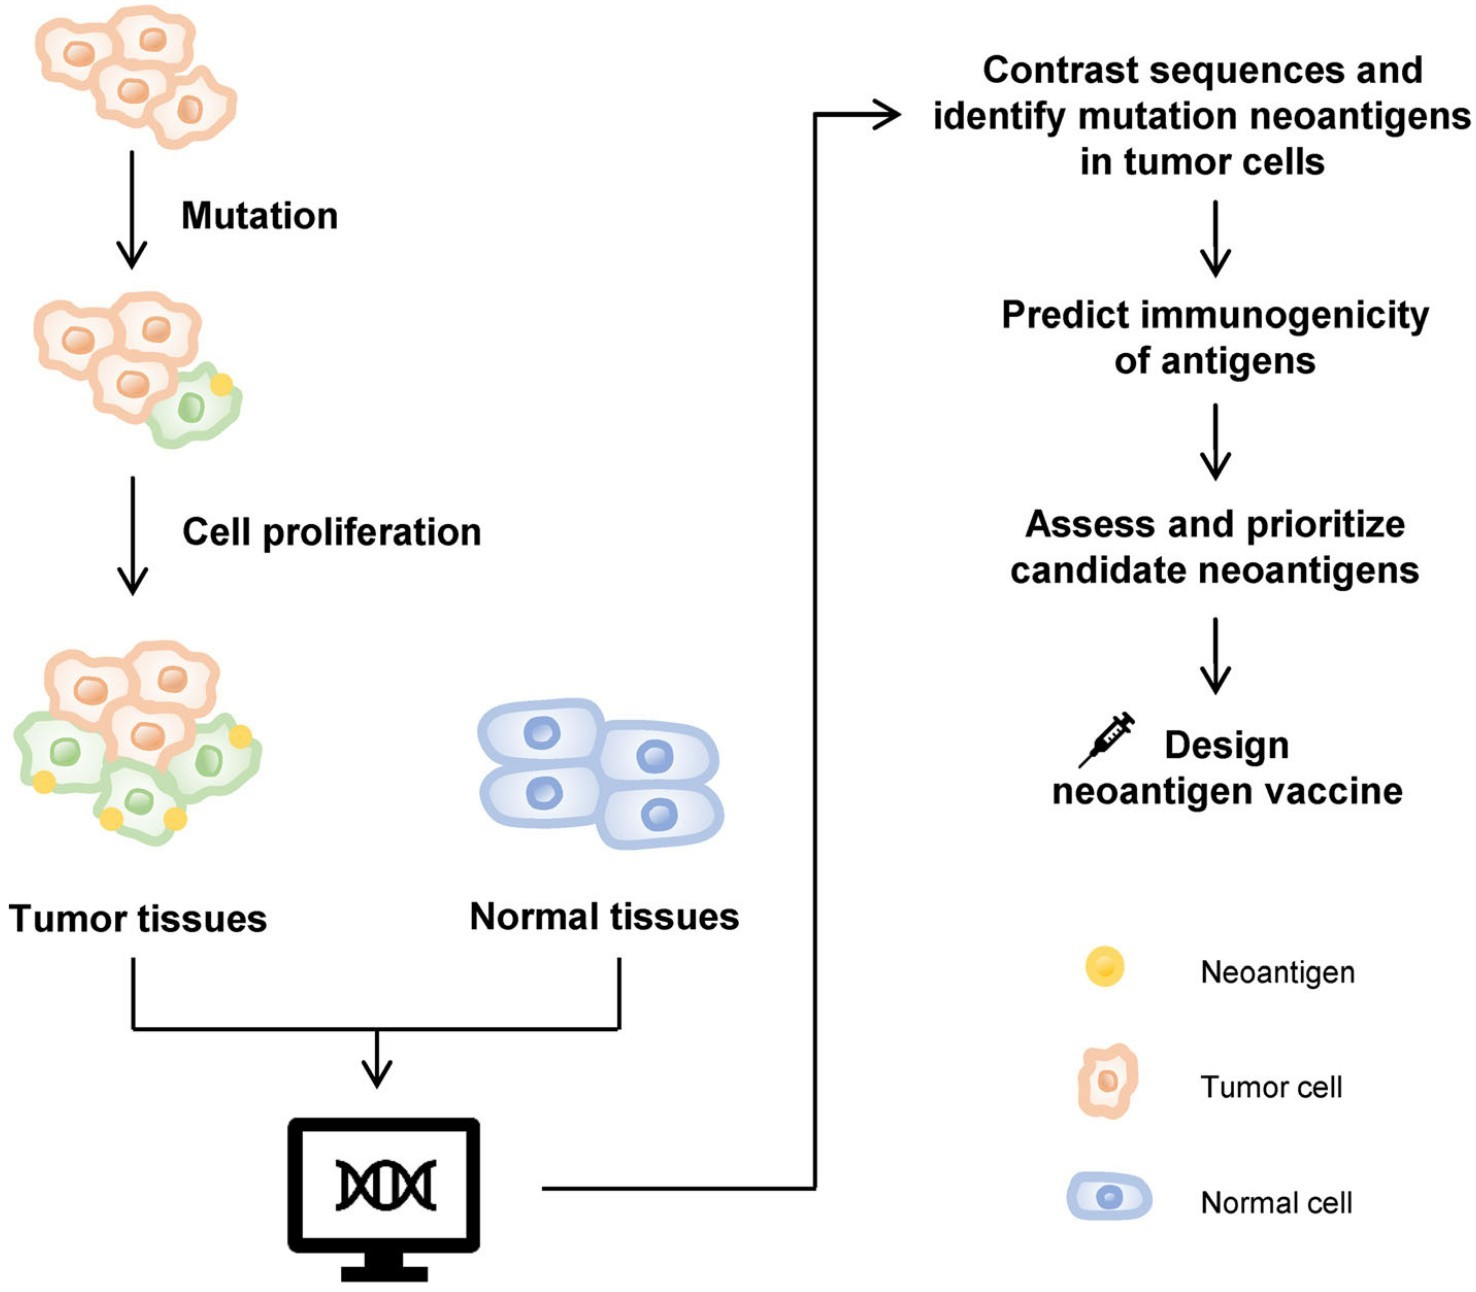
\includegraphics[width=0.6\textwidth]{../img/neoantigen/process}
			\caption{Personalized vaccines process for Cancer \cite{peng2019neoantigen}.}
		\end{figure}		
	\end{frame}
	%-------------------------------------------------------
	%-------------------------------------------------------
	
	%-------------------------------------------------------
	%-------------------------------------------------------
	\begin{frame}{Immunotherapy for Cancer}{Personalized Vaccines}	
		\begin{figure}
			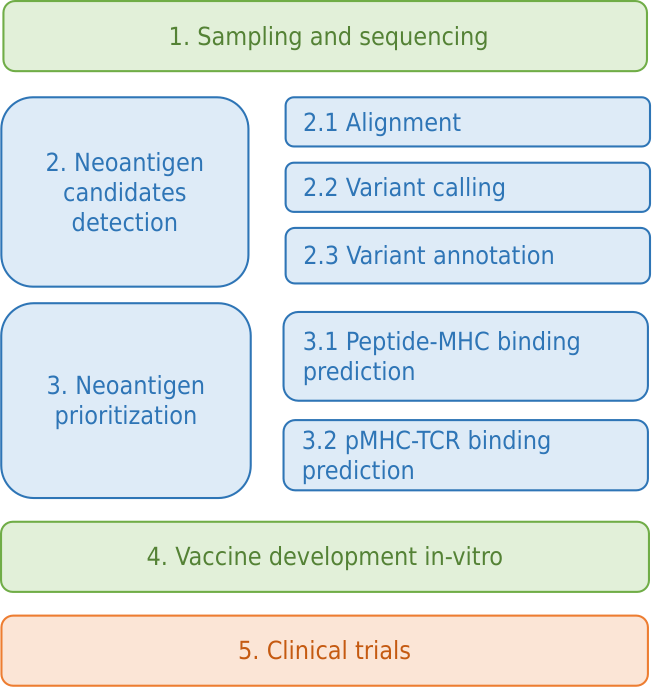
\includegraphics[width=0.5\textwidth]{../img/pipeline/pipeline_ingles}
			\caption{Personalized vaccines process for Cancer.}
		\end{figure}		
	\end{frame}
	%-------------------------------------------------------
	%-------------------------------------------------------
	
	
	
	%-------------------------------------------------------
	%-------------------------------------------------------
	\begin{frame}{pMHC binding prediction}{}		
		\begin{figure}[H]
			\centering
			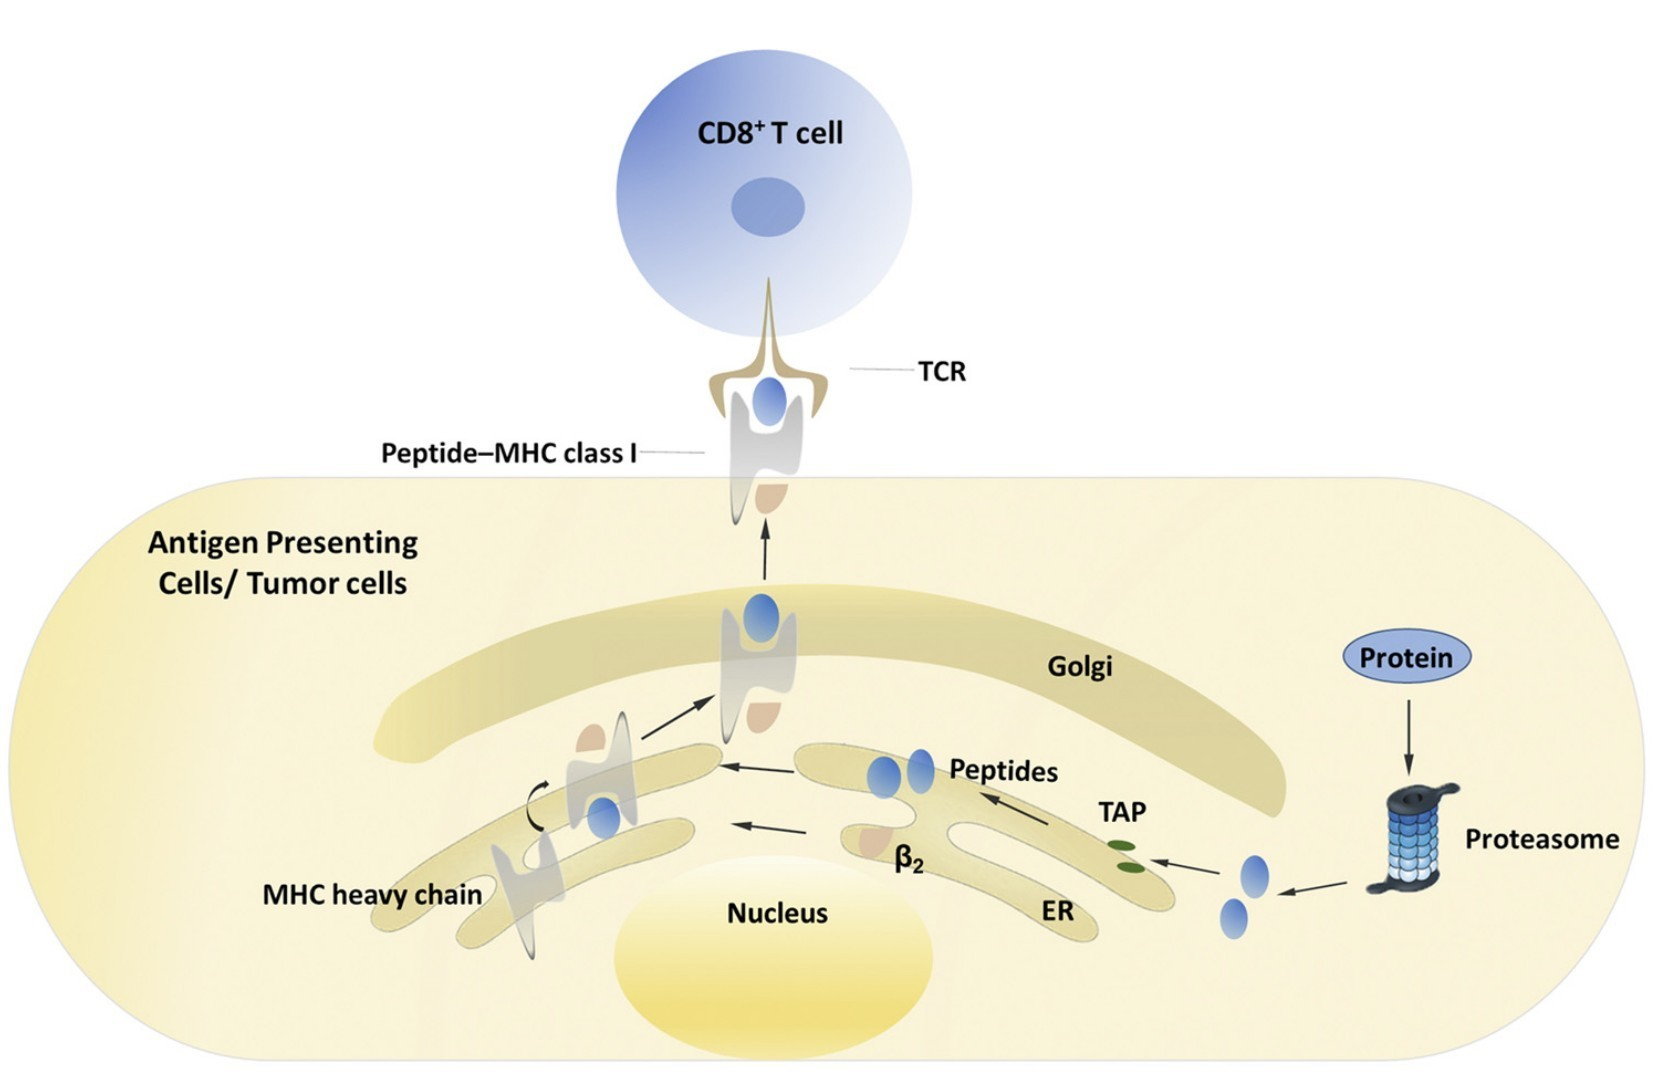
\includegraphics[width=0.9\textwidth]{../img/neoantigen/mhc1.jpg}
			\caption{pMHC presentation process in MHC class I \cite{zhang2019application}.}
			\label{fig:mhc1}
		\end{figure}	
	\end{frame}
	%-------------------------------------------------------
	%-------------------------------------------------------
	
	%%%%%%%%%%%%%%%%%%%%%%%%%%%%%%%%%%%%%%%%%%%%%%%%%%%%%%%%%%%%%%%%%%%%%%%%%%%%%%%%%%%%%%%%%%%%%%%%%%%%%%%%%%%%%%%%
	%%%%%%%%%%%%%%%%%%%%%%%%%%%%%%%%%%%%%%%%%%%%%%%%%%%%%%%%%%%%%%%%%%%%%%%%%%%%%%%%%%%%%%%%%%%%%%%%%%%%%%%%%%%%%%%%
	%%%%%%%%%%%%%%%%%%%%%%%%%%%%%%%%%%%%%%%%%%%%%%%%%%%%%%%%%%%%%%%%%%%%%%%%%%%%%%%%%%%%%%%%%%%%%%%%%%%%%%%%%%%%%%%%
	\subsection{Problem}
	%%%%%%%%%%%%%%%%%%%%%%%%%%%%%%%%%%%%%%%%%%%%%%%%%%%%%%%%%%%%%%%%%%%%%%%%%%%%%%%%%%%%%%%%%%%%%%%%%%%%%%%%%%%%%%%%
	%%%%%%%%%%%%%%%%%%%%%%%%%%%%%%%%%%%%%%%%%%%%%%%%%%%%%%%%%%%%%%%%%%%%%%%%%%%%%%%%%%%%%%%%%%%%%%%%%%%%%%%%%%%%%%%%
	%%%%%%%%%%%%%%%%%%%%%%%%%%%%%%%%%%%%%%%%%%%%%%%%%%%%%%%%%%%%%%%%%%%%%%%%%%%%%%%%%%%%%%%%%%%%%%%%%%%%%%%%%%%%%%%%
	
	%-------------------------------------------------------
	%-------------------------------------------------------
	\begin{frame}{Problem}{}
		
		\begin{block}{}
			\textbf{Less than 5\%} of detected neoantigens (peptides binded to MHC) succeed in activating the immune system \cite{de2020neoantigen}.
		\end{block}
		
		
		\begin{block}{}
			This is a \textbf{binary classification problem}. A peptide could be represented like: $p = \{ A, ... , Q \}$ and a MHC like: $q = \{ A, N, ... ,Q, E \}$. Finally, we need to know the probability of affinity between $p$ and $q$ (pMHC)
		\end{block}
		
		%	\begin{block}{Objectives}
			%		Proposed a method based on transformers and transfer learning for pMHC binding and	presentation prediction. 
			%	\end{block}	
		
	\end{frame}
	%-------------------------------------------------------
	%-------------------------------------------------------
	
	%-------------------------------------------------------
	%-------------------------------------------------------
	\begin{frame}{Problem}{}	
		\begin{figure}
			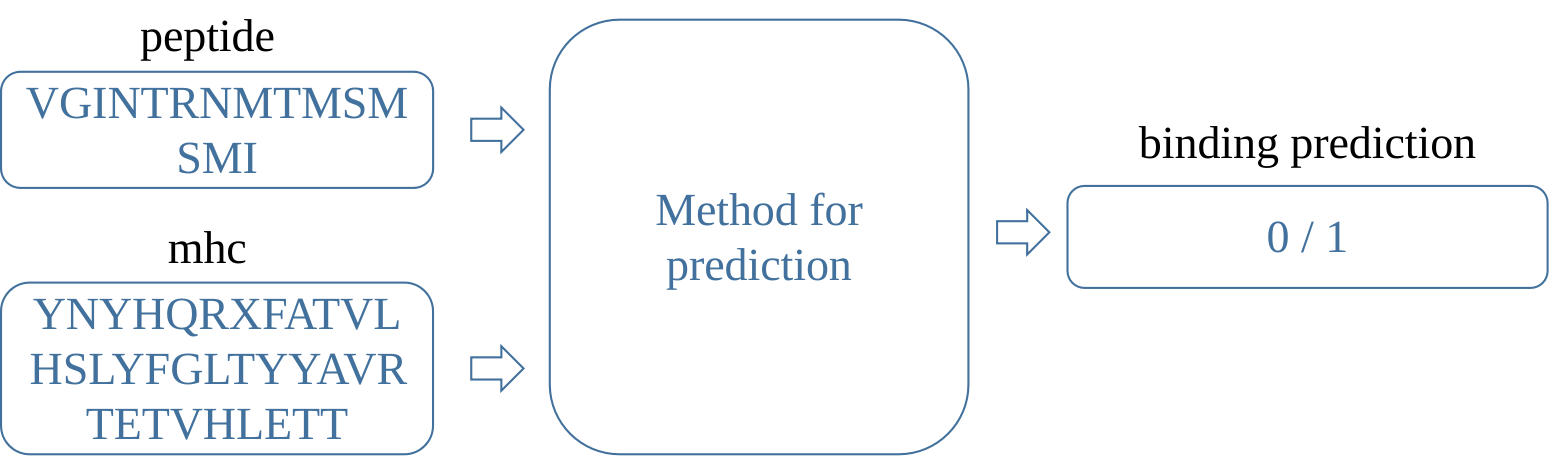
\includegraphics[width=0.97\textwidth]{../img/neoantigen/problem}
			\caption{pMHC binding prediction problem.}
		\end{figure}
	\end{frame}
	%-------------------------------------------------------
	%-------------------------------------------------------
	

	
	%%%%%%%%%%%%%%%%%%%%%%%%%%%%%%%%%%%%%%%%%%%%%%%%%%%%%%%%%%%%%%%%%%%%%%%%%%%%%%%%%%%%%%%%%%%%%%%%%%%%%%%%%%%%%%%%
	%%%%%%%%%%%%%%%%%%%%%%%%%%%%%%%%%%%%%%%%%%%%%%%%%%%%%%%%%%%%%%%%%%%%%%%%%%%%%%%%%%%%%%
	\section{Proposal}
	%%%%%%%%%%%%%%%%%%%%%%%%%%%%%%%%%%%%%%%%%%%%%%%%%%%%%%%%%%%%%%%%%%%%%%%%%%%%%%%%%%%%%%%%%%%%%%%%%%%%%%%%%%%%%%%%
	%%%%%%%%%%%%%%%%%%%%%%%%%%%%%%%%%%%%%%%%%%%%%%%%%%%%%%%%%%%%%%%%%%%%%%%%%%%%%%%%%%%%%%
	
		%%%%%%%%%%%%%%%%%%%%%%%%%%%%%%%%%%%%%%%%%%%%%%%%%%%%%%%%%%%%%%%%%%%%%%%%%%%%%%%%%%%%%%%%%%%%%%%%%%%%%%%%%%%%%%%%
	%%%%%%%%%%%%%%%%%%%%%%%%%%%%%%%%%%%%%%%%%%%%%%%%%%%%%%%%%%%%%%%%%%%%%%%%%%%%%%%%%%%%%%
	\subsection{Proposal}
	%%%%%%%%%%%%%%%%%%%%%%%%%%%%%%%%%%%%%%%%%%%%%%%%%%%%%%%%%%%%%%%%%%%%%%%%%%%%%%%%%%%%%%%%%%%%%%%%%%%%%%%%%%%%%%%%
	%%%%%%%%%%%%%%%%%%%%%%%%%%%%%%%%%%%%%%%%%%%%%%%%%%%%%%%%%%%%%%%%%%%%%%%%%%%%%%%%%%%%%%
	
	%-------------------------------------------------------
	%-------------------------------------------------------
	\begin{frame}{Proposal}{}
		
		\vspace{0.5cm}
		\begin{figure}[H]
			\centering
			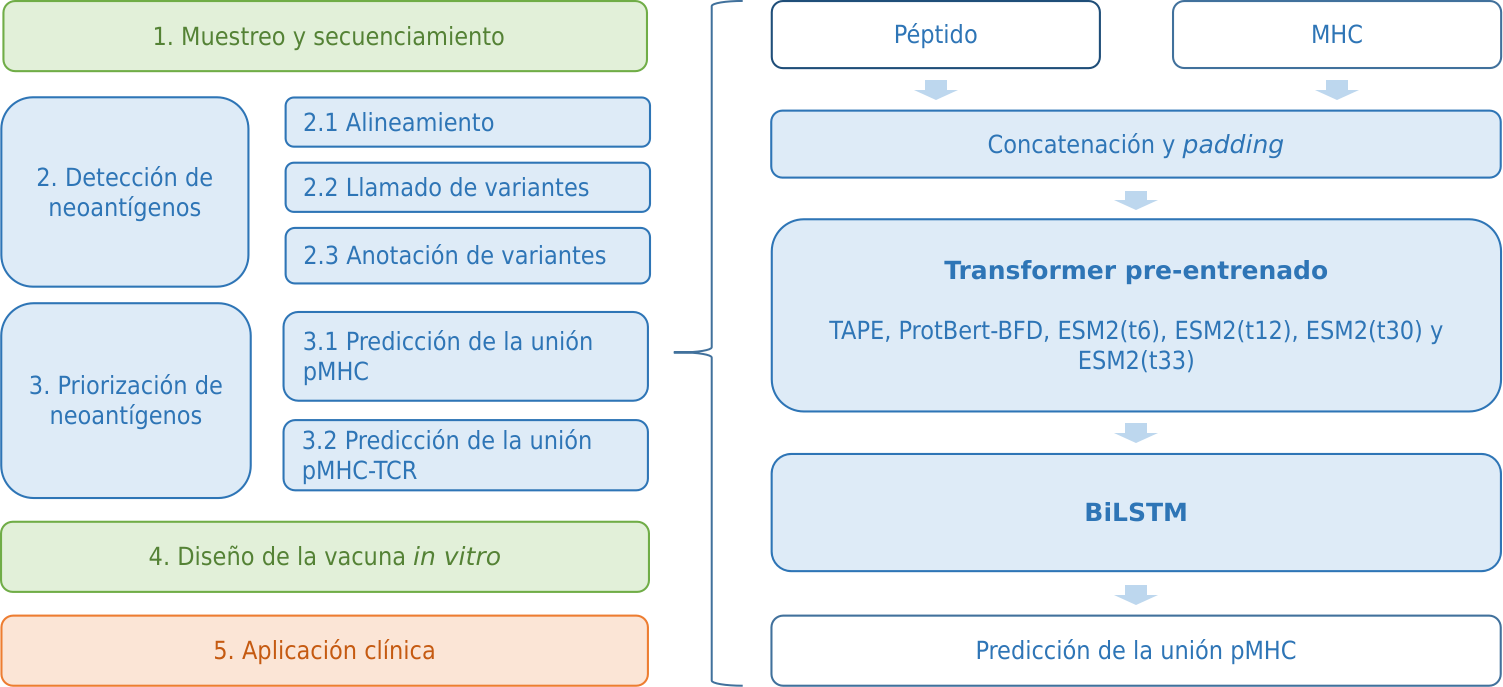
\includegraphics[width=\textwidth]{../img/proposal/proposal}	
			\caption{Proposal for pMHC binding prediction.}
			\label{fig:neo_det_seq}
		\end{figure}
	\end{frame}
	%-------------------------------------------------------
	%-------------------------------------------------------
	
	
	
	
%%%%%%%%%%%%%%%%%%%%%%%%%%%%%%%%%%%%%%%%%%%%%%%%%%%%%%%%%%%%%%%%%%%%%%%%%%%%%%%%%%%%%%%%%%%%%%%%%%%%%%%%%%%%%%%%
%%%%%%%%%%%%%%%%%%%%%%%%%%%%%%%%%%%%%%%%%%%%%%%%%%%%%%%%%%%%%%%%%%%%%%%%%%%%%%%%%%%%%%
\section{Experiments and Results}
%%%%%%%%%%%%%%%%%%%%%%%%%%%%%%%%%%%%%%%%%%%%%%%%%%%%%%%%%%%%%%%%%%%%%%%%%%%%%%%%%%%%%%%%%%%%%%%%%%%%%%%%%%%%%%%%
%%%%%%%%%%%%%%%%%%%%%%%%%%%%%%%%%%%%%%%%%%%%%%%%%%%%%%%%%%%%%%%%%%%%%%%%%%%%%%%%%%%%%%

%%%%%%%%%%%%%%%%%%%%%%%%%%%%%%%%%%%%%%%%%%%%%%%%%%%%%%%%%%%%%%%%%%%%%%%%%%%%%%%%%%%%%%%%%%%%%%%%%%%%%%%%%%%%%%%%
%%%%%%%%%%%%%%%%%%%%%%%%%%%%%%%%%%%%%%%%%%%%%%%%%%%%%%%%%%%%%%%%%%%%%%%%%%%%%%%%%%%%%%
\subsection{Databases}
%%%%%%%%%%%%%%%%%%%%%%%%%%%%%%%%%%%%%%%%%%%%%%%%%%%%%%%%%%%%%%%%%%%%%%%%%%%%%%%%%%%%%%%%%%%%%%%%%%%%%%%%%%%%%%%%
%%%%%%%%%%%%%%%%%%%%%%%%%%%%%%%%%%%%%%%%%%%%%%%%%%%%%%%%%%%%%%%%%%%%%%%%%%%%%%%%%%%%%%
	
%-------------------------------------------------------
%-------------------------------------------------------
\begin{frame}{Databases}{}
	
	Training: 539,019; Validation: 179,673; and Testing: 172,580.
	
	\begin{figure}[]
		\centering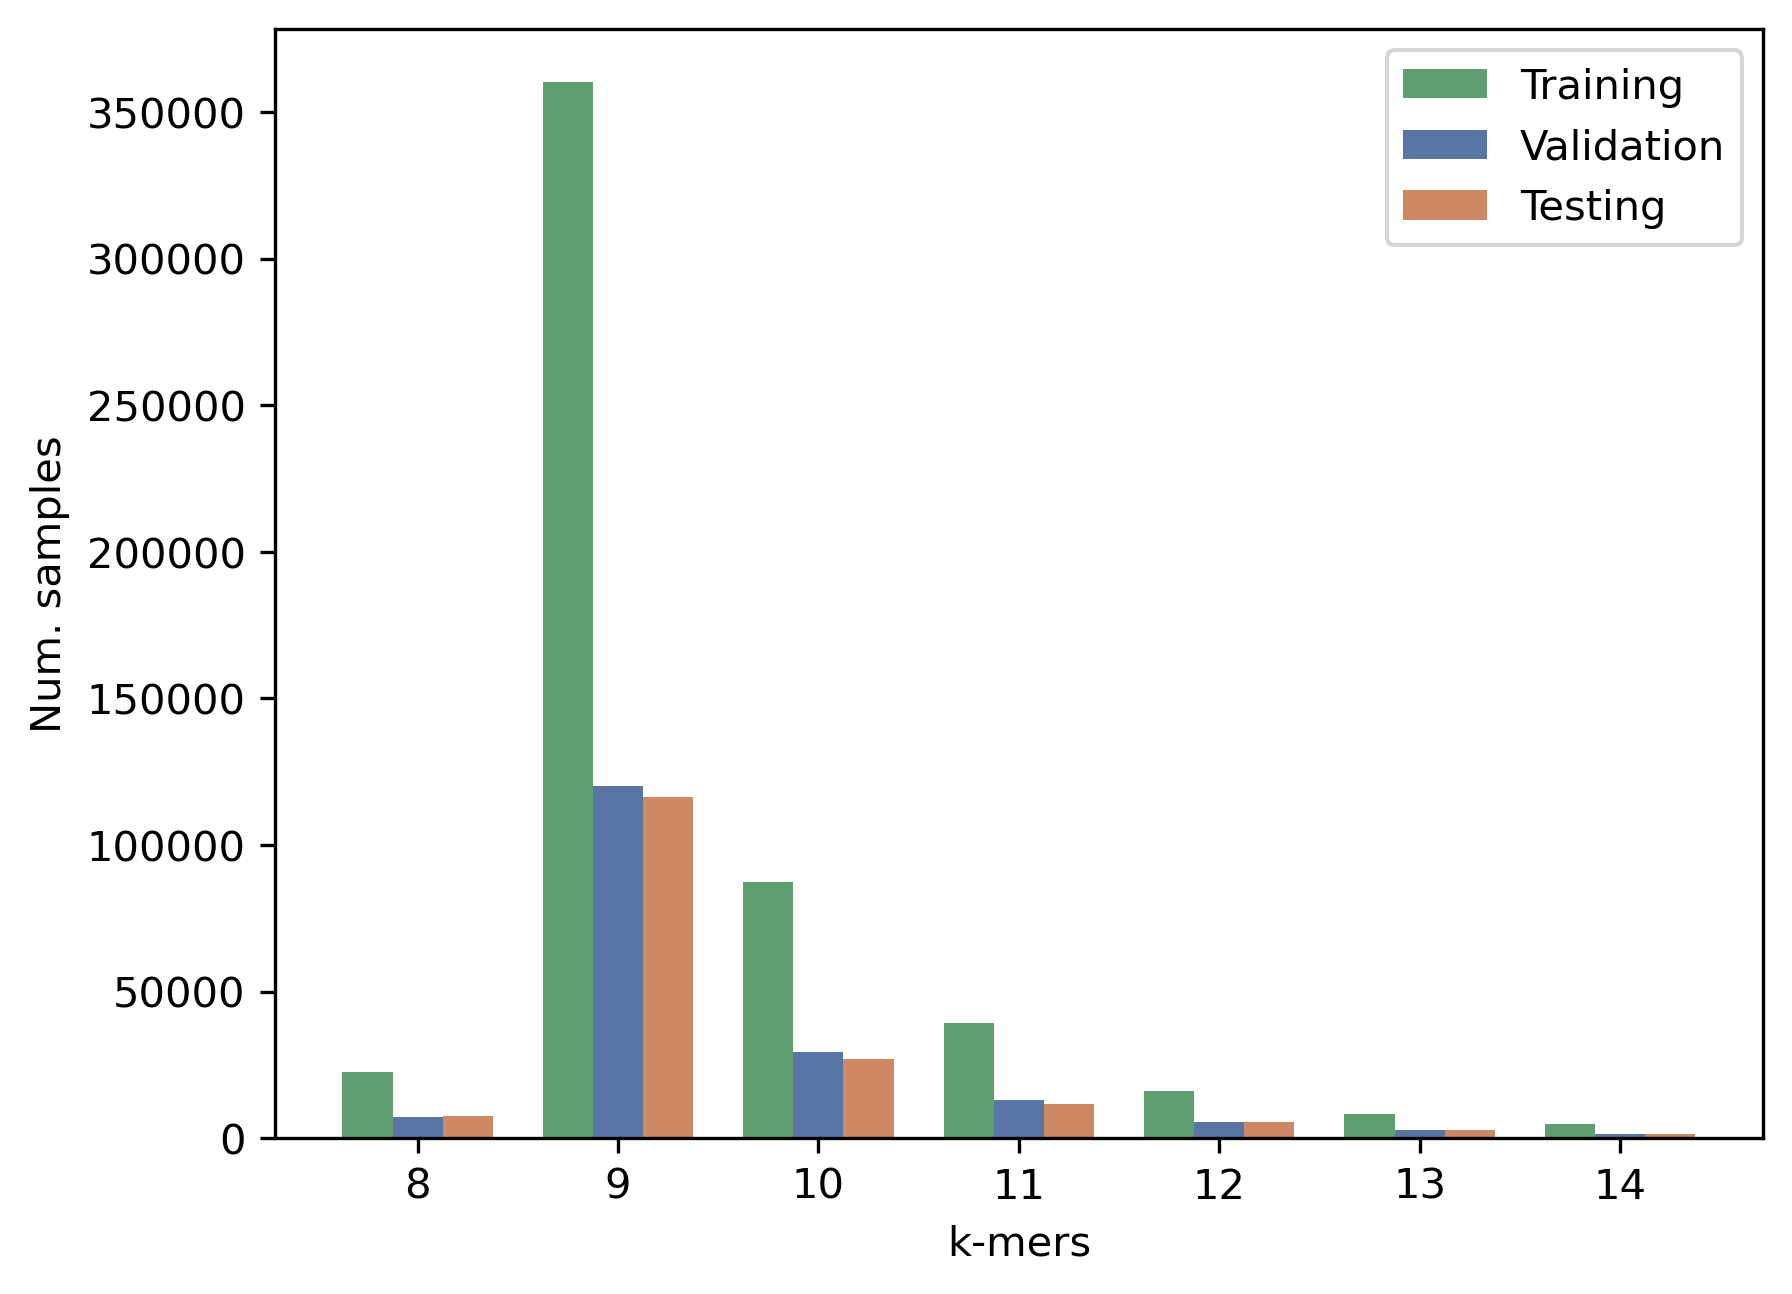
\includegraphics[width=0.7\textwidth]{../img/proposal/dataset_samples}
		\caption{
			Number of samples per k-mer.}
		\label{fig:samples}
	\end{figure}
	
\end{frame}
%-------------------------------------------------------
%-------------------------------------------------------
	
%%%%%%%%%%%%%%%%%%%%%%%%%%%%%%%%%%%%%%%%%%%%%%%%%%%%%%%%%%%%%%%%%%%%%%%%%%%%%%%%%%%%%%%%%%%%%%%%%%%%%%%%%%%%%%%%
%%%%%%%%%%%%%%%%%%%%%%%%%%%%%%%%%%%%%%%%%%%%%%%%%%%%%%%%%%%%%%%%%%%%%%%%%%%%%%%%%%%%%%
\subsection{Pre-trained models}
%%%%%%%%%%%%%%%%%%%%%%%%%%%%%%%%%%%%%%%%%%%%%%%%%%%%%%%%%%%%%%%%%%%%%%%%%%%%%%%%%%%%%%%%%%%%%%%%%%%%%%%%%%%%%%%%
%%%%%%%%%%%%%%%%%%%%%%%%%%%%%%%%%%%%%%%%%%%%%%%%%%%%%%%%%%%%%%%%%%%%%%%%%%%%%%%%%%%%%%	
	
%-------------------------------------------------------
%-------------------------------------------------------
\begin{frame}{Pre-trained models}{}
	
\begin{table}
	\centering
	\caption{Differences between TAPE, ProtBert-DFB, and ESM2. HS: \textit{Hidden size}; AH: \textit{Attention heads}.}
	\label{tab:pretrained}%
	\setlength{\tabcolsep}{0.5em} % for the horizontal padding
	{\renewcommand{\arraystretch}{1.5}% for the vertical padding
		\footnotesize
		\begin{tabular}{llrrrrr}
			
			\textbf{Model}   & \textbf{BD} & \textbf{Samples} & \textbf{Layers} & \textbf{HS} & \textbf{AH} & \textbf{Params.} \\
			\hline
			TAPE             & Pfam             & 30M                   & 12              & 768                  & 12                       & 92M                 \\
			ProtBert-BFD     & BFD              & 2122M                 & 30              & 1024                 & 16                       & 420M                \\
			ESM2(t6)  & Uniref50         & 60M                   & 6               & 320                  & 20                       & 8M                  \\
			ESM2(t12)  & Uniref50         & 60M                   & 12              & 480                  & 20                       & 35M                 \\
			ESM2(t30) & Uniref50         & 60M                   & 30              & 640                  & 20                       & 150M                \\
			ESM2(t33)  & Uniref50         & 60M                   & 33              & 1280                 & 20                       & 650M               \\
			
	\end{tabular}}
	
\end{table}
	
\end{frame}
%-------------------------------------------------------
%-------------------------------------------------------
	

%%%%%%%%%%%%%%%%%%%%%%%%%%%%%%%%%%%%%%%%%%%%%%%%%%%%%%%%%%%%%%%%%%%%%%%%%%%%%%%%%%%%%%%%%%%%%%%%%%%%%%%%%%%%%%%%
%%%%%%%%%%%%%%%%%%%%%%%%%%%%%%%%%%%%%%%%%%%%%%%%%%%%%%%%%%%%%%%%%%%%%%%%%%%%%%%%%%%%%%
\subsection{Results}
%%%%%%%%%%%%%%%%%%%%%%%%%%%%%%%%%%%%%%%%%%%%%%%%%%%%%%%%%%%%%%%%%%%%%%%%%%%%%%%%%%%%%%%%%%%%%%%%%%%%%%%%%%%%%%%%
%%%%%%%%%%%%%%%%%%%%%%%%%%%%%%%%%%%%%%%%%%%%%%%%%%%%%%%%%%%%%%%%%%%%%%%%%%%%%%%%%%%%%%	

%-------------------------------------------------------
%-------------------------------------------------------
\begin{frame}{Results}{(Training for 3 epochs)}
	\begin{figure}
		\centering		
			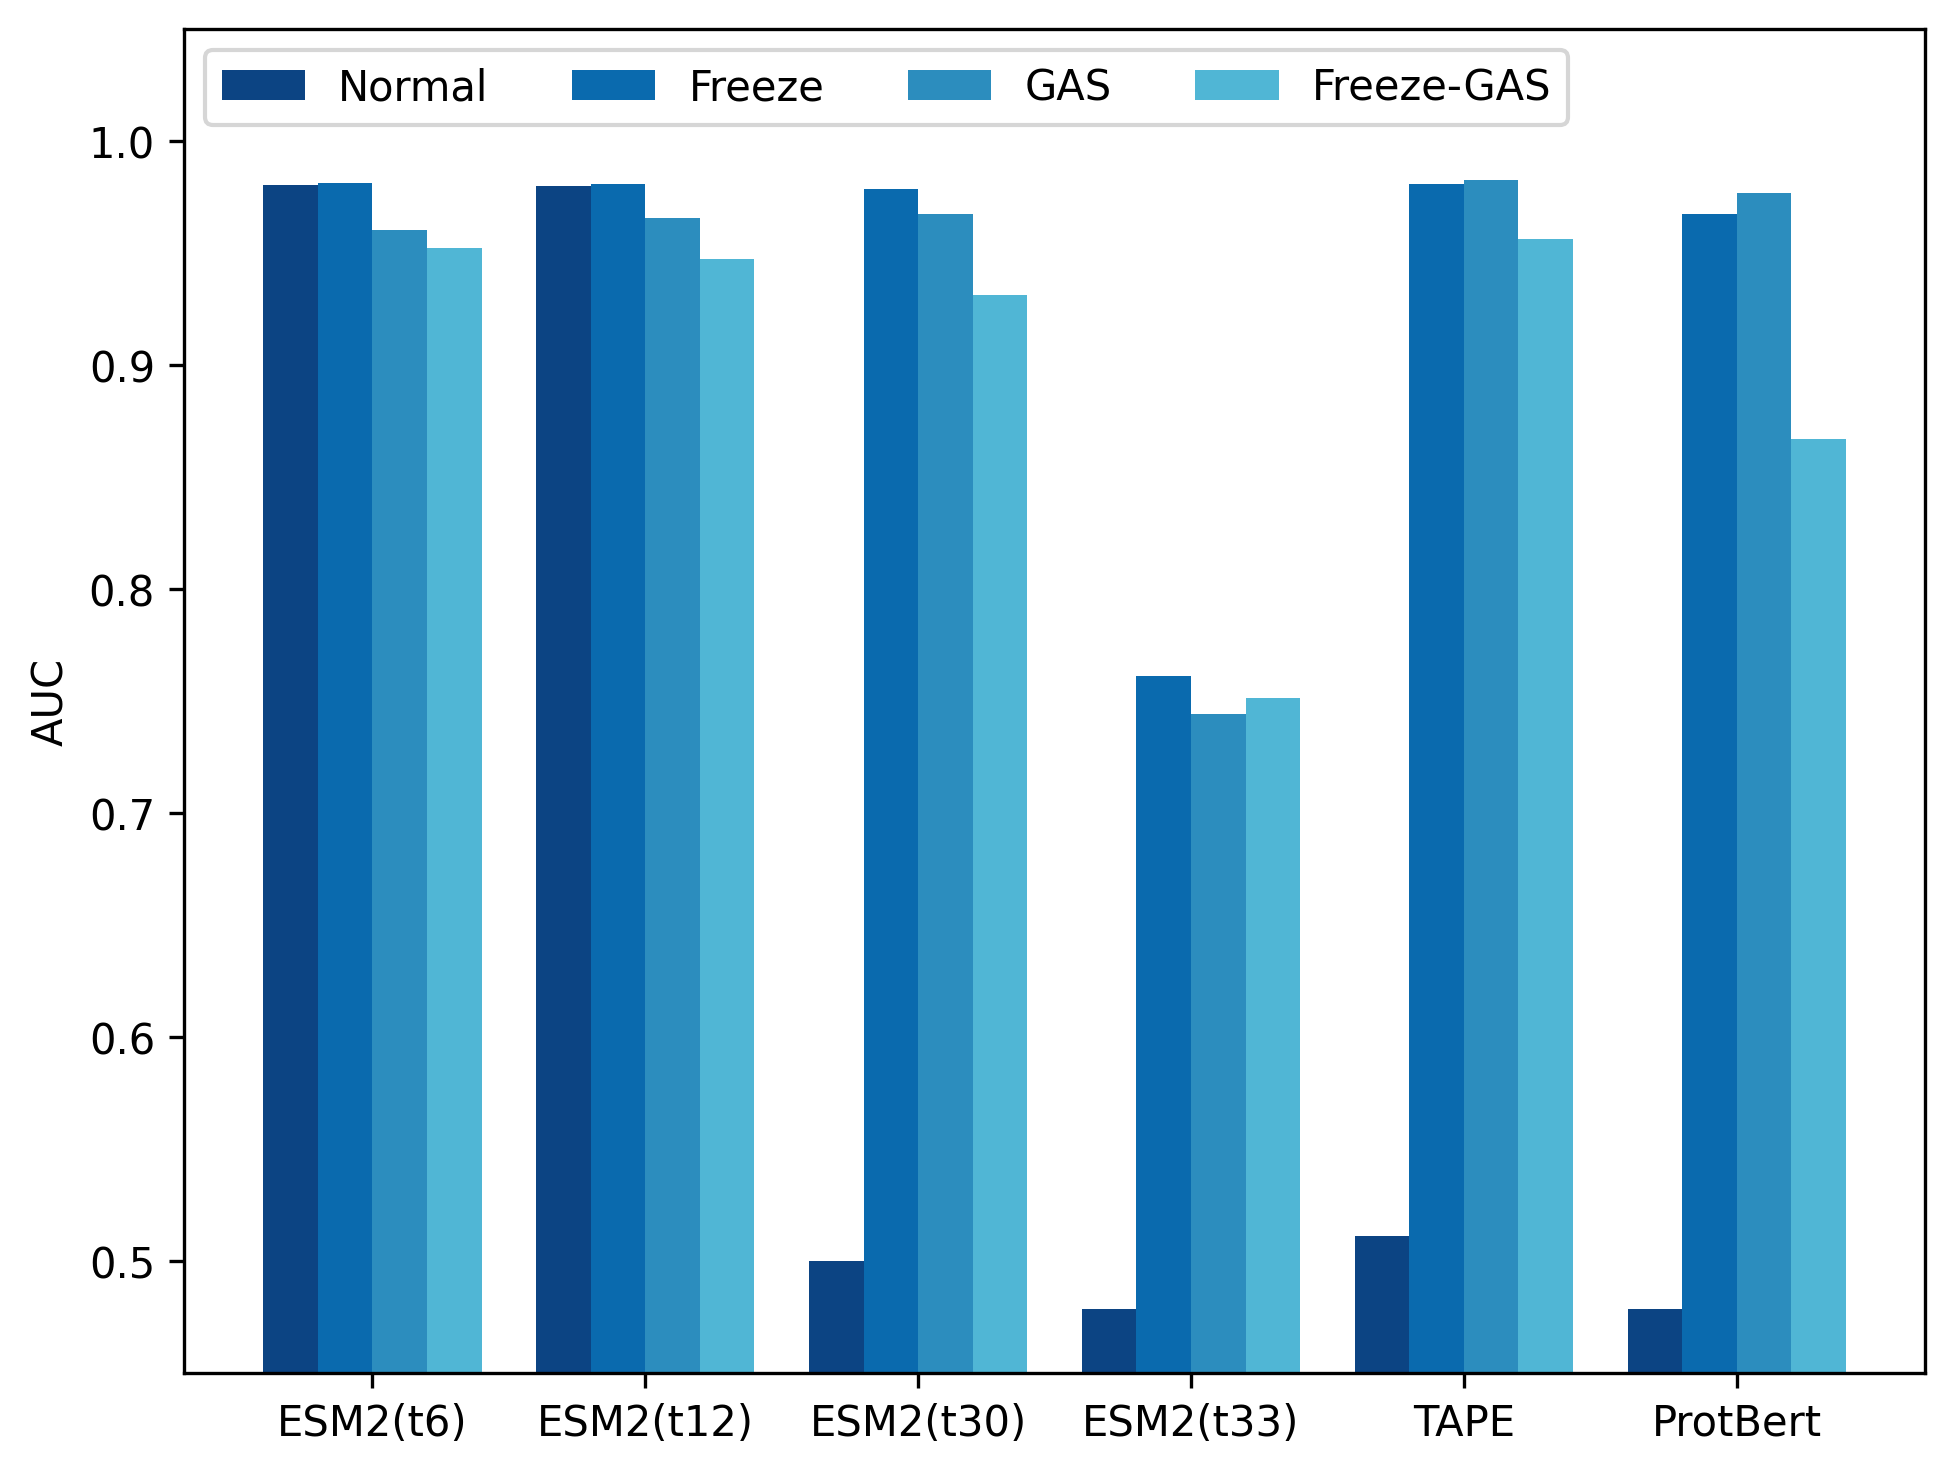
\includegraphics[width=0.7\textwidth]{../img/results/metrics_comparion_by_model}			
		\caption{Comparative analysis of Area Under the Curve (AUC) in Transformer model architectures using various training methodologies.}
		\label{fig:comparison_3_3pochs}
	\end{figure}
\end{frame}
%-------------------------------------------------------
%-------------------------------------------------------
	
	
%-------------------------------------------------------
%-------------------------------------------------------
\begin{frame}{Results}{Vanish gradient problem}
	\centering
	Gradients for ESM2(t6)
	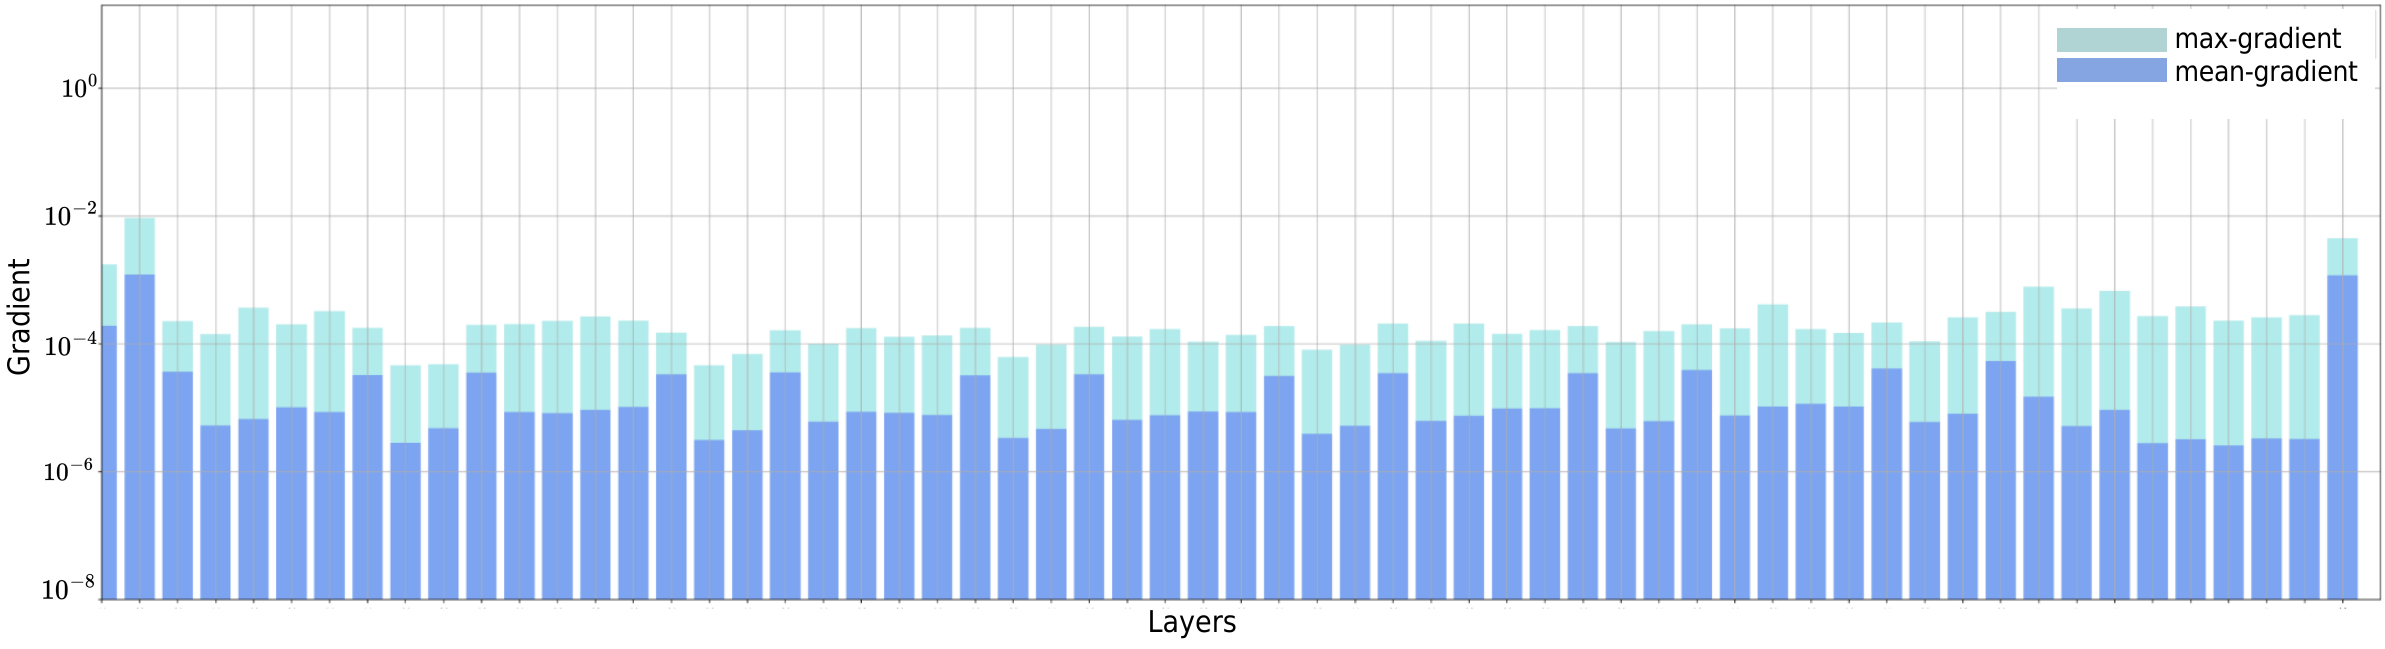
\includegraphics[width=\textwidth]{../img/results/t6_epoch0}
	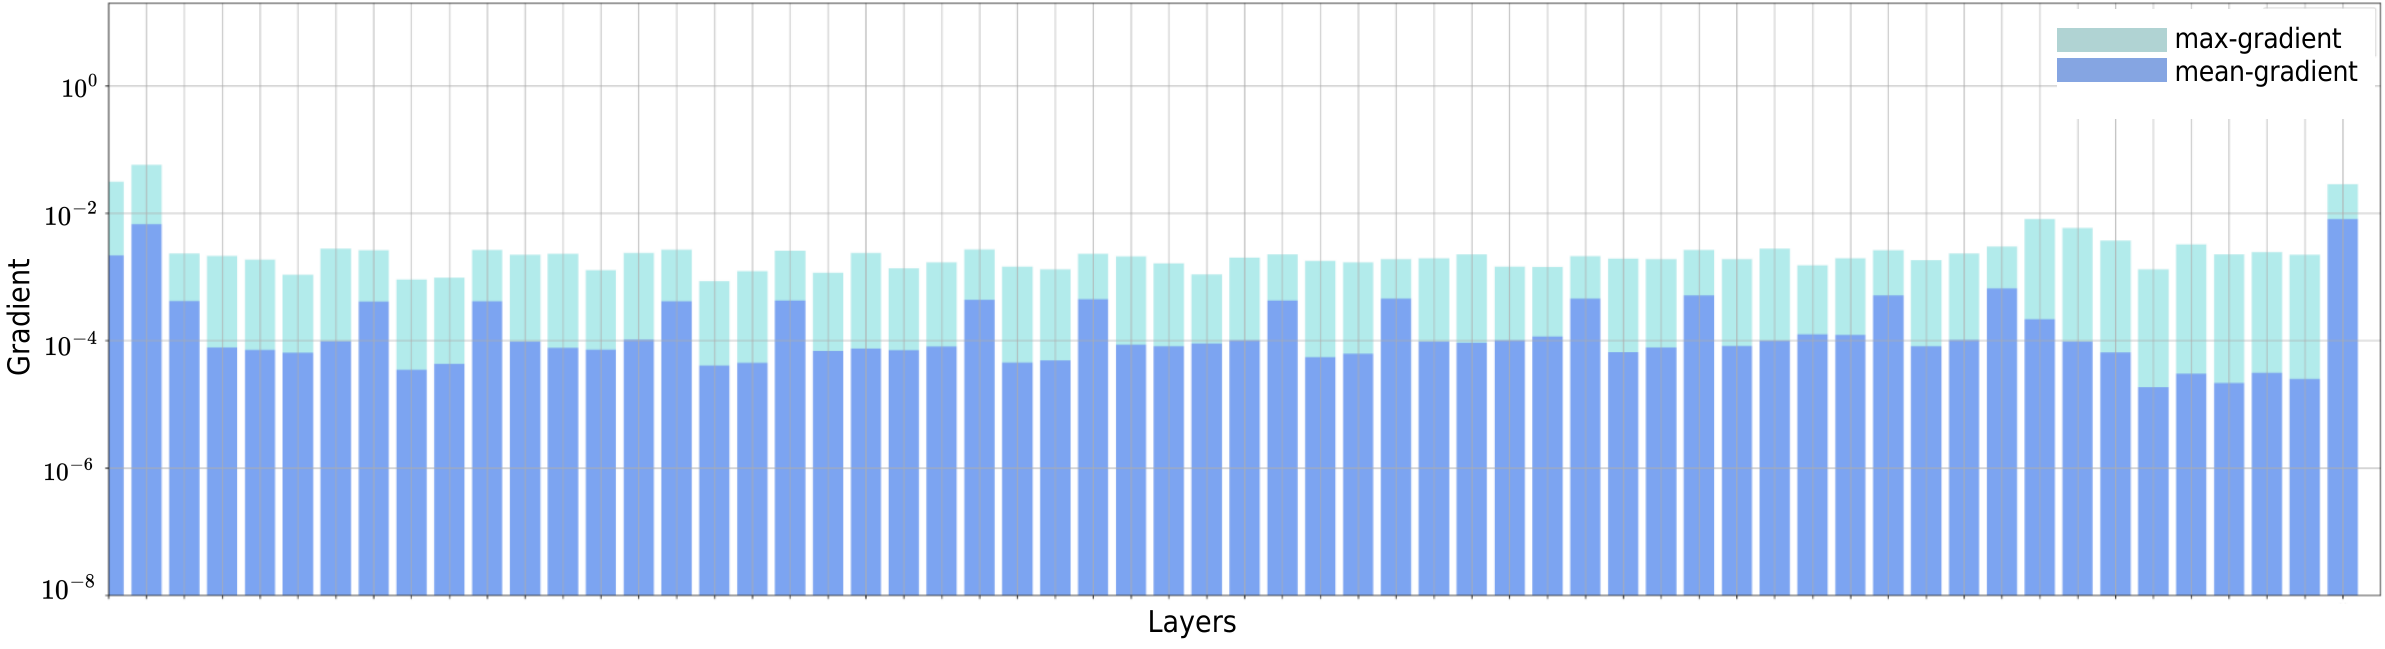
\includegraphics[width=\textwidth]{../img/results/t6_epoch3}
\end{frame}
%-------------------------------------------------------
%-------------------------------------------------------

%-------------------------------------------------------
%-------------------------------------------------------
\begin{frame}{Results}{Vanish gradient problem}
	\centering
	Gradients for ESM2(t30)
	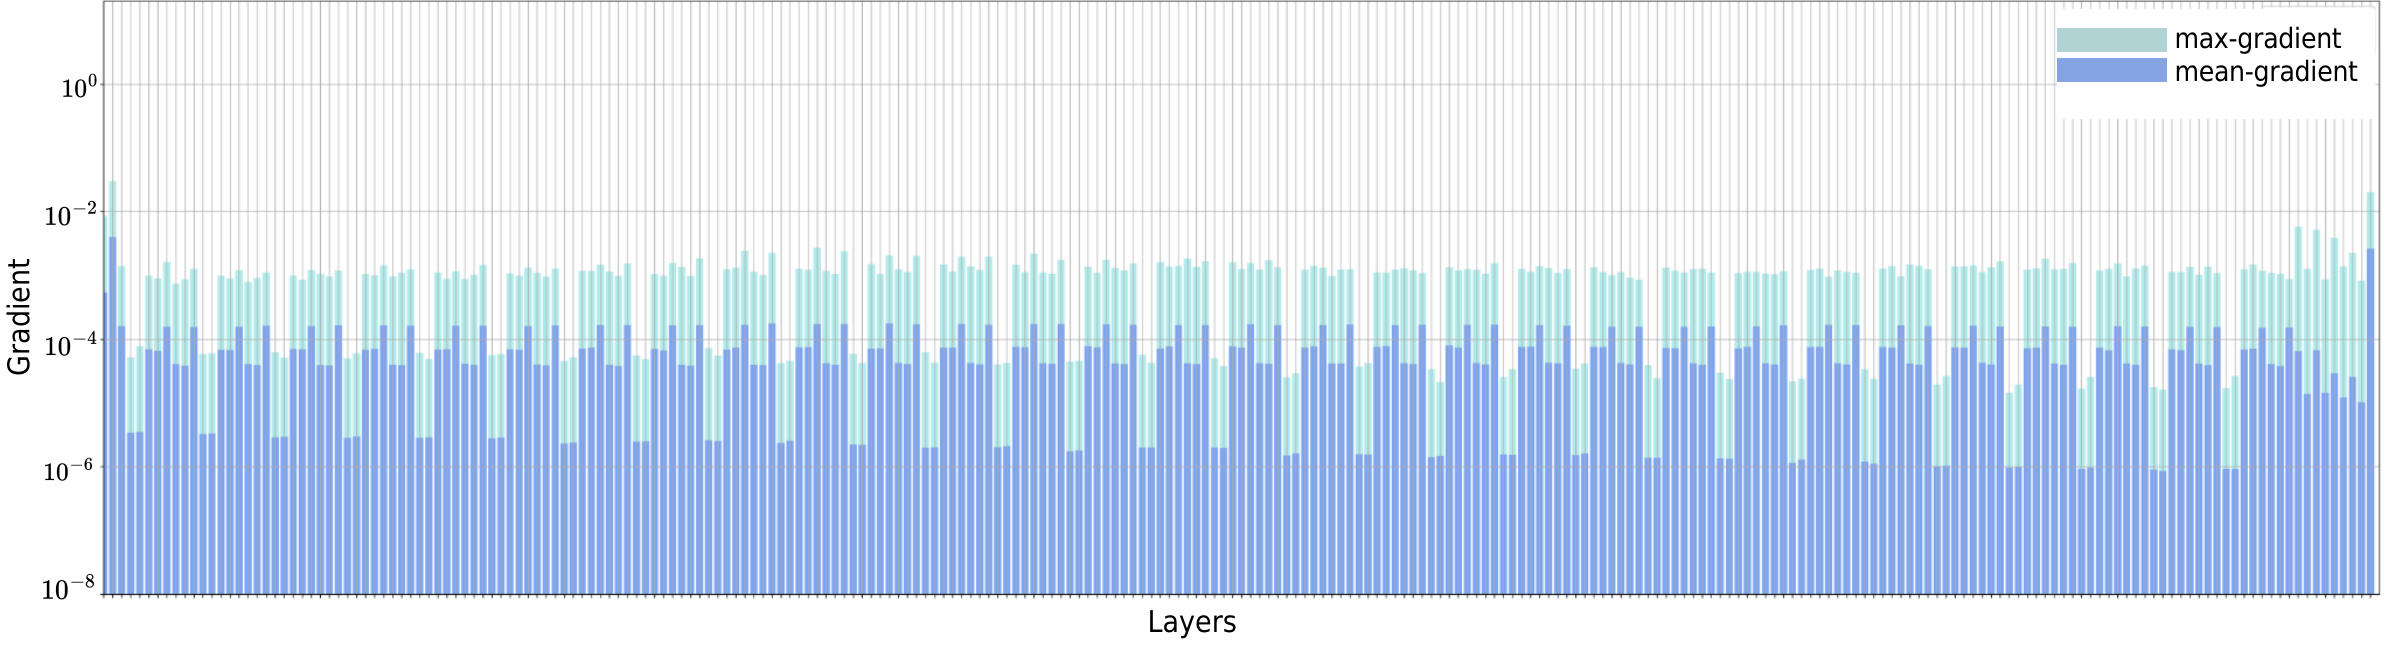
\includegraphics[width=\textwidth]{../img/results/t30_epoch0}
	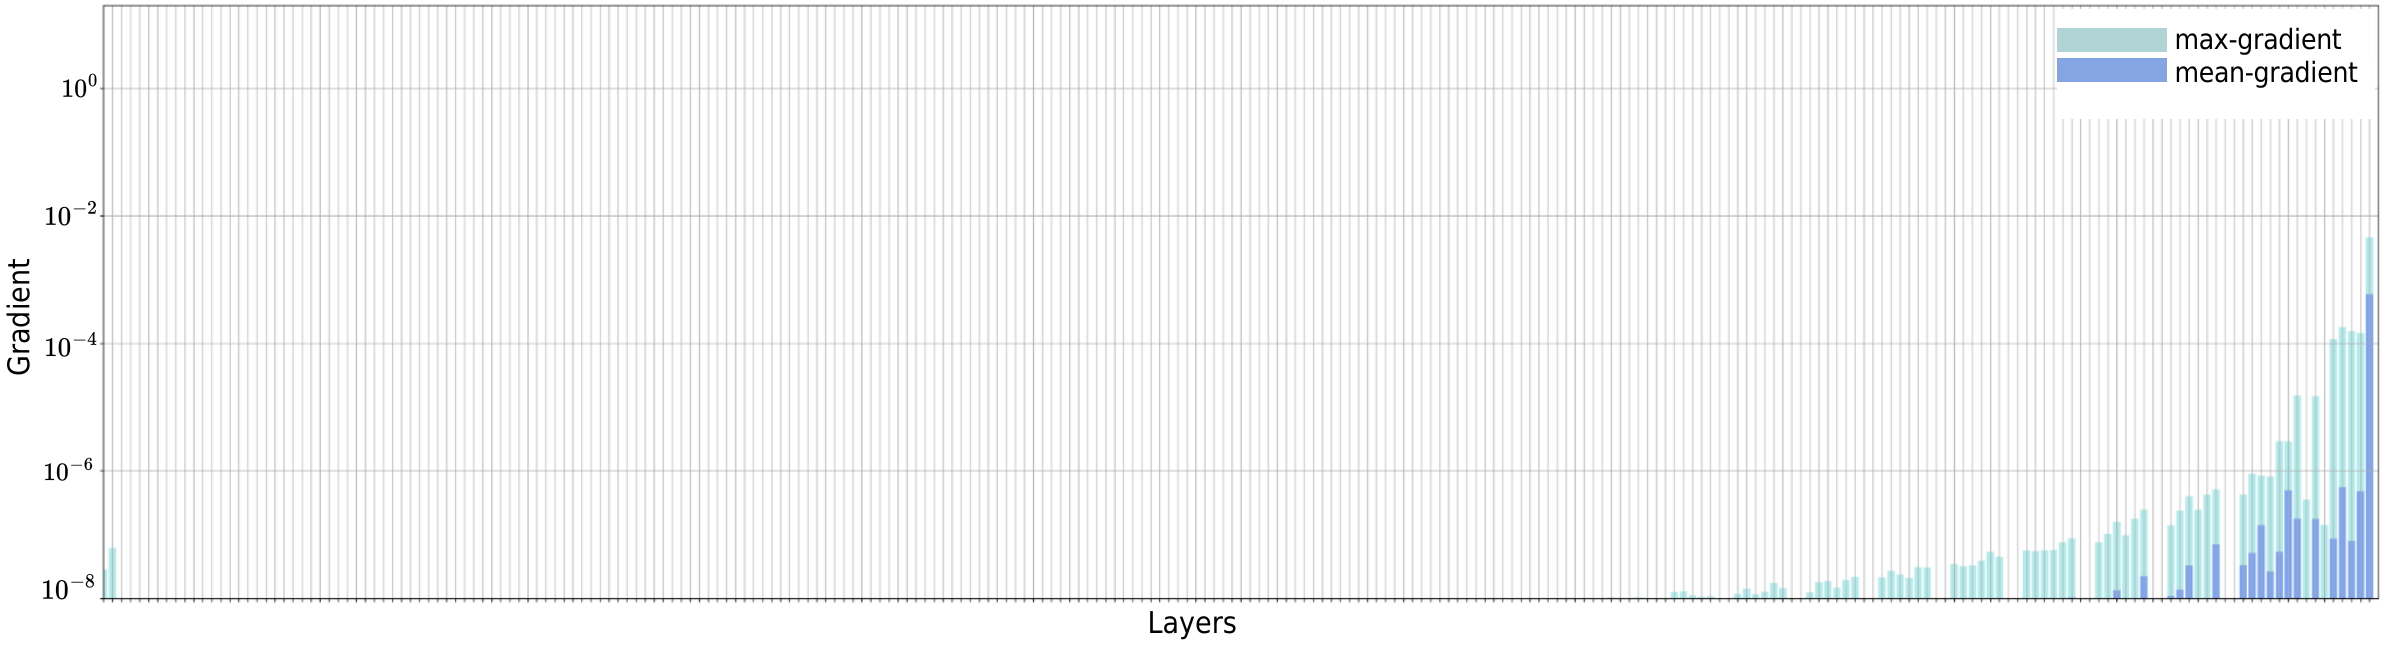
\includegraphics[width=\textwidth]{../img/results/t30_epoch3}
\end{frame}
%-------------------------------------------------------
%-------------------------------------------------------

%-------------------------------------------------------
%-------------------------------------------------------
\begin{frame}{Results}{Comparison (Training for 30 epochs)}
\begin{table}[]
	\centering
	\setlength{\tabcolsep}{0.5em} % for the horizontal padding
	{\renewcommand{\arraystretch}{1.5}% for the vertical padding
	\scriptsize
	\begin{tabular}{lllllll} 
		\textbf{}            & \textbf{Accuracy} & \textbf{Precision} & \textbf{Recall} & \textbf{F1-score} & \textbf{AUC}    & \textbf{MCC}    \\ \hline
		ESM2(t6)-Normal             & 0.9390            & 0.9333             & \textbf{0.9453} & 0.9392            & 0.9797          & 0.8780                    \\
		ESM2(t6)-Freeze      & \textbf{0.9401}   & \textbf{0.9398}    & 0.9402          & \textbf{0.9400}   & \textbf{0.9830} & \textbf{0.8802}             \\
		ESM2(t6)-GAS         & 0.9366            & 0.9322             & 0.9413          & 0.9368            & 0.9818          & 0.8732                     \\
		ESM2(t6)-Freeze-GAS  & 0.9354            & 0.9326             & 0.9383          & 0.9355            & 0.9813          & 0.8708                    \\ \hline
		ESM2(t30)-Normal            & -                 & -                  & -               & -                 & -               & -                                 \\
		ESM2(t30)-Freeze     & \textbf{0.9393}   & 0.9304             & \textbf{0.9493} & \textbf{0.9397}   & 0.9787          & \textbf{0.8787}           \\
		ESM2(t30)-GAS        & 0.9346            & \textbf{0.9337}    & 0.9352          & 0.9345            & 0.9808          & 0.8691                    \\
		ESM2(t30)-Freeze-GAS & 0.9363            & 0.9319             & 0.9411          & 0.9365            & \textbf{0.9818} & 0.8726                    \\ \hline
		TAPE-Normal                 & -                 & -                  & -               & -                 & -               & -                                  \\
		TAPE-Freeze          & 0.9395            & \textbf{0.9404}    & 0.9382          & 0.9393            & 0.9815          & 0.8790                      \\
		TAPE-GAS             & \textbf{0.9415}   & 0.9352             & \textbf{0.9484} & \textbf{0.9418}   & \textbf{0.9841} & \textbf{0.8831}            \\
		TAPE-Freeze-GAS      & 0.9359            & 0.9297             & 0.9428          & 0.9362            & 0.9820          & 0.8719               \\     
	\end{tabular}}
\end{table}
\end{frame}
%-------------------------------------------------------
%-------------------------------------------------------


%-------------------------------------------------------
%-------------------------------------------------------
\begin{frame}{Results}{Comparison with state-of-art tools}
	\begin{figure}
		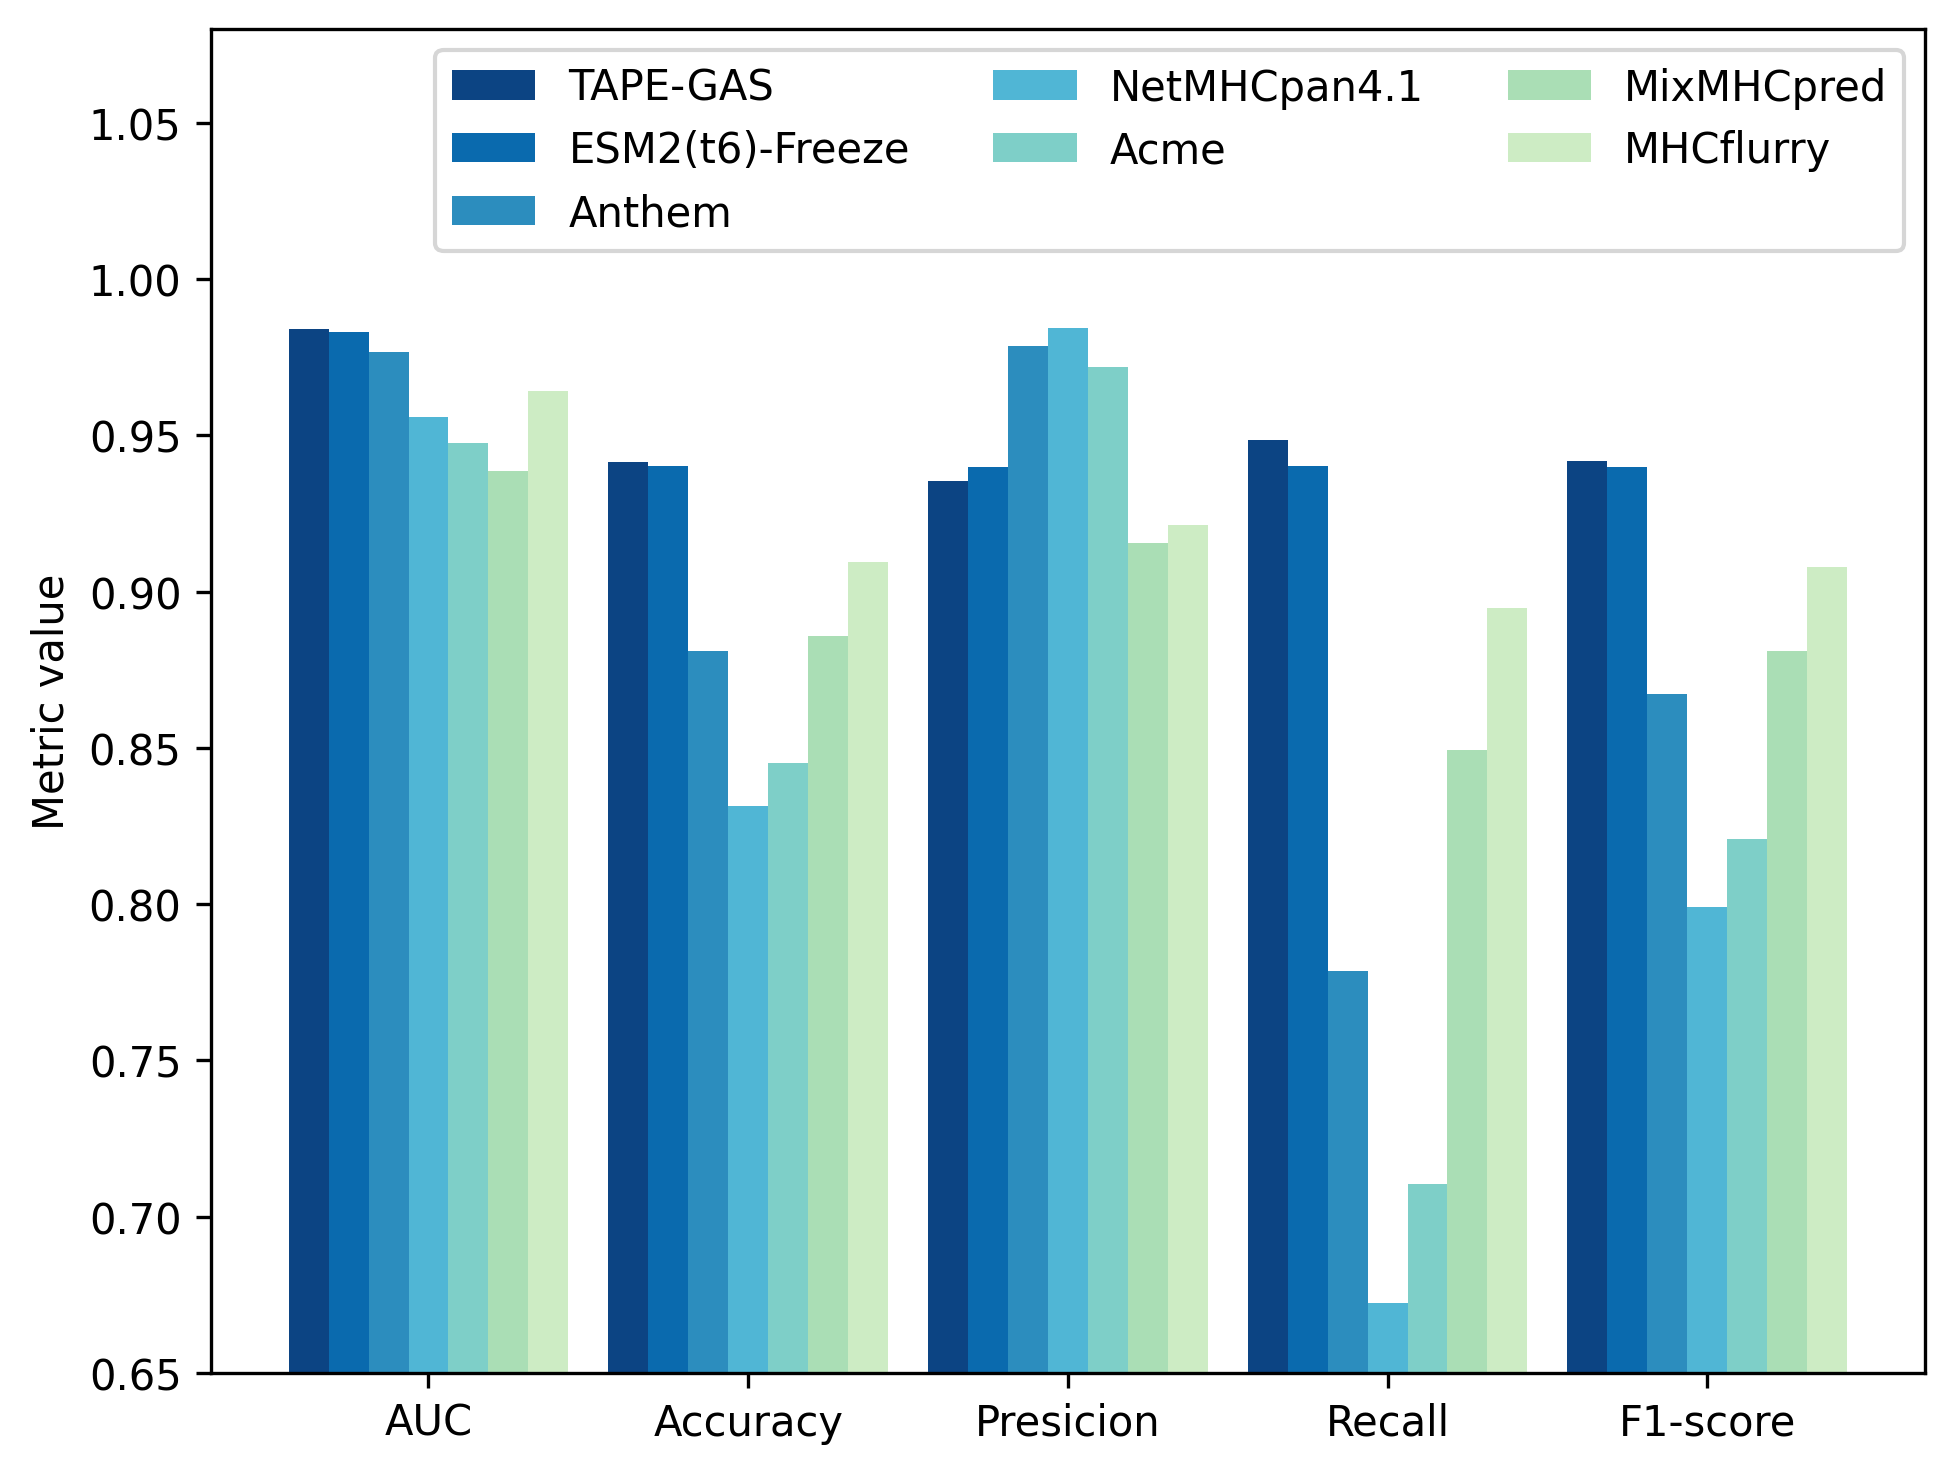
\includegraphics[width=0.8\textwidth]{../img/results/metrics_comparison}
		\caption{The AUC values for TAPE-GAS and ESM2(t6) trained for 30 epochs, in comparison to state-of-the-art methods.}
		\label{fig:comparison_final}
	\end{figure}
\end{frame}
%-------------------------------------------------------
%-------------------------------------------------------

%-------------------------------------------------------
%-------------------------------------------------------
\begin{frame}{Results}{Comparison with state-of-art tools}
	\begin{figure}
		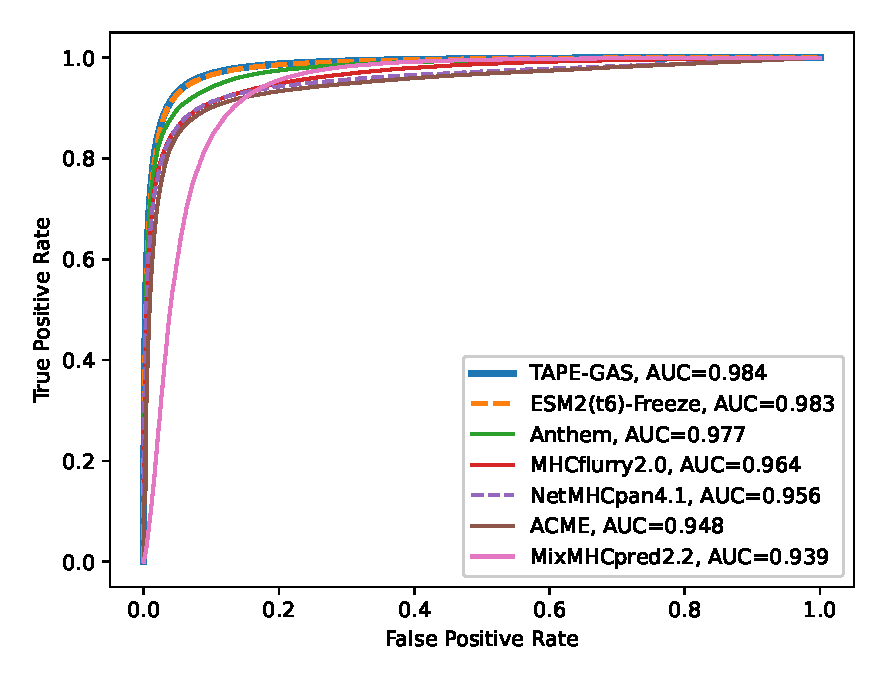
\includegraphics[width=0.8\textwidth]{../img/results/ROC_comparison}
		\caption{ROC curves for TAPE-GAS and ESM2(t6) trained for 30 epochs, in comparison to state-of-the-art methods.}
	\end{figure}
\end{frame}
%-------------------------------------------------------
%-------------------------------------------------------

%-------------------------------------------------------
%-------------------------------------------------------
\begin{frame}{Results}{Comparison with state-of-art tools}
	\begin{table}[]
		\centering
		\caption{Performance evaluation of Transformer models TAPE-GAS and ESM2(t6)-Freeze, trained for 30 epochs, against Anthem, NetMHCpan4.1, ACME, MixMHCpred2.2, and MhcFlurry2.0.}
		\label{tab:final_comparison}
		\setlength{\tabcolsep}{0.5em} % for the horizontal padding
		{\renewcommand{\arraystretch}{1.5}% for the vertical padding
			\scriptsize
		\begin{tabular}{lllllll} 
			& \textbf{Accuracy} & \textbf{Precision} & \textbf{Recall} & \textbf{F1-score} & \textbf{AUC}    & \textbf{MCC}    \\ \hline
			TAPE-GAS        & \textbf{0.9415}   & 0.9352             & \textbf{0.9484} & \textbf{0.9418}   & \textbf{0.9841} & \textbf{0.8831} \\
			ESM2(t6)-Freeze & \textbf{0.9401}   & 0.9398             & \textbf{0.9402} & \textbf{0.9400}   & \textbf{0.9830} & \textbf{0.8802} \\
			
			Anthem          & 0.8811            & \textbf{0.9786}    & 0.7787          & 0.8673            & 0.9768          & 0.7785          \\
			NetMHCpan4.1    & 0.8312            & \textbf{0.9844}    & 0.6724          & 0.7991            & 0.9557          & 0.6982          \\
			
			ACME            & 0.8452            & 0.9717             & 0.7105          & 0.8208            & 0.9476          & 0.7165          \\
			MixMHCpred2.2   & 0.8857            & 0.9155             & 0.8493          & 0.8811            & 0.9386          & 0.7733          \\
			MhcFlurry2.0    & 0.9093            & 0.9211             & 0.8948          & 0.9078            & 0.9642          & 0.8189 \\         
		\end{tabular}}
	\end{table}
\end{frame}
%-------------------------------------------------------
%-------------------------------------------------------

	
	%%%%%%%%%%%%%%%%%%%%%%%%%%%%%%%%%%%%%%%%%%%%%%%%%%%%%%%%%%%%%%%%%%%%%%%%%%%%%%%%%%%%%%%%%%%%%%%%%%%%%%%%%%%%%%%%
	%%%%%%%%%%%%%%%%%%%%%%%%%%%%%%%%%%%%%%%%%%%%%%%%%%%%%%%%%%%%%%%%%%%%%%%%%%%%%%%%%%%%%%
	\section{Discussion and Conclusions}
	%%%%%%%%%%%%%%%%%%%%%%%%%%%%%%%%%%%%%%%%%%%%%%%%%%%%%%%%%%%%%%%%%%%%%%%%%%%%%%%%%%%%%%%%%%%%%%%%%%%%%%%%%%%%%%%%
	%%%%%%%%%%%%%%%%%%%%%%%%%%%%%%%%%%%%%%%%%%%%%%%%%%%%%%%%%%%%%%%%%%%%%%%%%%%%%%%%%%%%%%
		%%%%%%%%%%%%%%%%%%%%%%%%%%%%%%%%%%%%%%%%%%%%%%%%%%%%%%%%%%%%%%%%%%%%%%%%%%%%%%%%%%%%%%%%%%%%%%%%%%%%%%%%%%%%%%%%
	%%%%%%%%%%%%%%%%%%%%%%%%%%%%%%%%%%%%%%%%%%%%%%%%%%%%%%%%%%%%%%%%%%%%%%%%%%%%%%%%%%%%%%
	\subsection{Discussion}
	%%%%%%%%%%%%%%%%%%%%%%%%%%%%%%%%%%%%%%%%%%%%%%%%%%%%%%%%%%%%%%%%%%%%%%%%%%%%%%%%%%%%%%%%%%%%%%%%%%%%%%%%%%%%%%%%
	%%%%%%%%%%%%%%%%%%%%%%%%%%%%%%%%%%%%%%%%%%%%%%%%%%%%%%%%%%%%%%%%%%%%%%%%%%%%%%%%%%%%%%
	
	
		
	%-------------------------------------------------------
	%-------------------------------------------------------
	\begin{frame}{Discussion}{}
		
		\begin{block}{Fine-tuning ESM2 models}
		The most favorable results were obtained with the smallest model, \textbf{ESM2(t6)}. we believe is not sufficiently large for ESM2(t33), a model boasting 650 million parameters. 
		\end{block}
	
	\begin{block}{}
		Another potential reason could be attributed to the use of \textbf{Rotary Position Embedding (RoPE)} used instead of absolute positional encoding.
	\end{block}
			
	\end{frame}
	%-------------------------------------------------------
	%-------------------------------------------------------
	
		%-------------------------------------------------------
	%-------------------------------------------------------
	\begin{frame}{Discussion}{}
		
	
		\begin{block}{Layer Freezing and GAS}
			This approach involves locking the Transformer model while updating only the BiLSTM parameters. This method is generally well-suited to accelerate the training process, even though it may lead to a slight sacrifice in performance. 
		\end{block}
	
				\begin{block}{}
			 Surprisingly, \textbf{for ESM2 models, this methodology yielded the best results, while for TAPE and ProtBert-BFD, it yielded the expected outcomes}.
		\end{block}
	\end{frame}
	%-------------------------------------------------------
	%-------------------------------------------------------
	
	
	%-------------------------------------------------------
	%-------------------------------------------------------
	\begin{frame}{Discussion}{}
		
		
		\begin{block}{TAPE, ProtBert-BFD and ESM2}
		\textbf{ProtBert-BFD got the worst result} despite this model were pre-trained with the largest dataset BFD with 2122M samples. We believe, this result is caused by the noisy information and sequence mistakes in BFD dataset.
		\end{block}
		
		\begin{block}{}
		\textbf{TAPE achieved the best results}. TAPE models were pre-trained using the Pfam dataset, it is derived from UniProtKB and \textbf{selectively includes sequences belonging to Reference Proteomes rather than  the entire UniProtKB}
		\end{block}
	
		\begin{block}{}
			\textbf{ESM2(t6) achieved results that closely rival TAPE}. ESM2(t6) comprises only 8 million parameters, compared to 92 million parameters of TAPE.
		\end{block}
	\end{frame}
	%-------------------------------------------------------
	%-------------------------------------------------------
	


	
	%-------------------------------------------------------
	%-------------------------------------------------------
	\begin{frame}[allowframebreaks]
		\frametitle{References}
		%\bibliographystyle{amsalpha}
		\bibliographystyle{IEEEtran}
		\bibliography{../bibliography_thesis.bib}
	\end{frame}
	%-------------------------------------------------------
	%-------------------------------------------------------
	
	%-------------------------------------------------------
	%-------------------------------------------------------
	\if\mycmd1 % MY THEME
	\1{
		{\1
			\begin{frame}[plain,noframenumbering]
				%\finalpage{Thank you}
				\begin{figure}[]
					\centering
					
\includegraphics[width=\textwidth,height=0.7\textheight,keepaspectratio]{../img/question.png}
					%\label{img:mot2}
					%\caption{Image example in 2 gray levels.}
				\end{figure}
		\end{frame}}
		\else % CS THEME
		\begin{frame}{Questions?}
			\begin{figure}[]
				\centering
				
\includegraphics[width=\textwidth,height=0.7\textheight,keepaspectratio]{../img/question.png}
				%\label{img:mot2}
				%\caption{Image example in 2 gray levels.}
			\end{figure}
			
		\end{frame}
		\fi
		%-------------------------------------------------------
		%-------------------------------------------------------
		
		
	\end{document}